\subsection{Partie préconditionneur}
La factorisation LU en algèbre linéaire dense est une méthode pour factoriser une matrice $A$ en deux matrices $L$ et $U$.
%
$L$ est une matrice triangulaire inférieure, toutes les valeurs au-dessus de la diagonale sont nulles.
%
Symétriquement, toutes les valeurs de $U$ en dessous de la diagonale sont nulles.
%
Le principal intérêt ce cette factorisation est de trouver $x$ dans les équations du type $Ax=y$.
%
Cette équation est transformée en deux équations $L.x_{tmp}=y$ et $U.x=x_{tmp}$.
%
La méthode utilisée pour résoudre un système composée d'une matrice triangulaire est triviale.
%
Il suffit de résoudre chaque équation ligne par ligne en commençant par la ligne qui n'as qu'une seule valeur non nulle.
%
Ensuite il faut résoudre la ligne avec deux valeurs non nulles dont une des inconnues provient de la solution précédente, et ainsi de suite jusqu'à la dernière ligne.
%
Cet algorithme est purement séquentiel mais des travaux existent pour exploiter du parallélisme dans certaines phases de l'algorithme~\cite{plasma_lu}.



La factorisation LU d'une matrice $A$ creuse donne deux matrices triangulaires denses $L$ et $U$.
%
Or, dans le cas où la matrice creuse à factoriser est trop grande, ces deux matrices ne peuvent pas tenir en mémoire.
%
C'est pourquoi en algèbre linéaire creuse, on utilise une version altérée de cette factorisation que l'on appelle factorisation incomplète, ou {\em ILU}\footnote{Incomplete LU}.
%
L'algorithme ILU est similaire à l'algorithme LU mais le remplissage est limité par des conditions définies par l'algorithme.
%
Le motif des matrices $L$ et $U$ reste similaire au motif de la matrice $A$.
%
Il y a du parallélisme dans l'algorithme ILU, certaines lignes peuvent être factorisées en parallèle et ce parallélisme se représente naturellement sous la forme d'un graphe de tâches (Fig.~\ref{fig:example_3_dag}).
%
Chaque tâche représente la factorisation d'une ligne de la matrice et les dépendances entre les tâches sont données par le motif de la matrice.
%
En effet, pour factoriser la ligne $i$, nous devons factoriser toutes les lignes $j$ inférieures à $i$ tel que l'entrée $(i,j)$ de la matrice soit non nulle (Fig.~\ref{fig:example_2_matrix}).
%
Donc, à partir du motif des valeurs non-nulles de la matrice, nous pouvons facilement construire le graphe de tâche:
%
la tâche $i$ corresponds à la ligne $i$ de la matrice, la liste des taches prédécesseurs de la tâche $i$ est donnée par l'index de colonne des valeurs non-nulles avant la diagonale dans la ligne $i$ et la liste des taches successeurs de la tâche $i$ est donnée par l'index de ligne des valeurs non-nulles au-dessous de la diagonale de la colonne $i$.

\begin{figure}[!ht]
     \begin{center}
        \subfigure[Un réservoir à 4 cellules]{%
          \label{fig:example_1_res}
          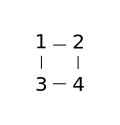
\includegraphics[width=0.32\textwidth]{example_1_res}
        }%
        \subfigure[Une matrice avec 4 cellules]{%
          \label{fig:example_2_matrix}
          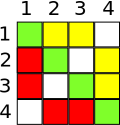
\includegraphics[width=0.32\textwidth]{example_2_matrix}
        }%
        \subfigure[Un DAG à 4 cellules]{%
          \label{fig:example_3_dag}
          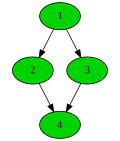
\includegraphics[width=0.32\textwidth]{example_3_dag}
        }%
    \end{center}
    \caption{Trois représentations d'un réservoir. Les éléments en rouge dans la matrice déterminent les dépendances dans le DAG.}
    \label{fig:exemple_3_dag}
\end{figure}

En résumé, le parallélisme de l'algorithme ILU peut se représenter sous la forme d'un graphe de tâches.
%
Chaque tâche représente la factorisation d'une ligne... ce qui est bien petit.
%
En fait, la plupart des runtimes mettront plus de temps à ordonnancer la tâche que la tâche mettra à factoriser une ligne.


Les problèmes rencontrés pour paralléliser la factorisation incomplète ainsi que les résolutions triangulaires associées d'une matrice creuse sont des problèmes qui représentent bien la difficulté que l'on peut rencontrer avec une parallélisation à grain fin.
%
La description à grain fin de ces algorithmes est naturelle, mais en pratique, une simple parallélisation utilisant Intel TBB ou OpenMP ne donnera pas de bonnes performances à cause du faible coût de calcul d'une tâche.
%
On appelle ça le problème de granularité.
%
Pour résoudre ce problème, les tâches doivent devenir plus grosses, nous devons factoriser plusieurs lignes à l'intérieur d'une tâche.
%
Mais le choix de ces lignes n'est pas trivial, il faut limiter l'impact sur le parallélisme et ne pas changer le résultat final.
%
Une méthode générique a été développée durant la thèse et sera expliquée plus loin dans ce document.
